%\documentclass[mathserif]{beamer}
\documentclass[handout]{beamer}
%\usetheme{Goettingen}
%\usetheme{Warsaw}
\usetheme{Singapore}



%\usetheme{Frankfurt}
%\usetheme{Copenhagen}
%\usetheme{Szeged}
%\usetheme{Montpellier}
%\usetheme{CambridgeUS}
%\usecolortheme{}
%\setbeamercovered{transparent}
\usepackage[english, activeacute]{babel}
\usepackage[utf8]{inputenc}
\usepackage{amsmath, amssymb}
\usepackage{dsfont}
\usepackage{graphics}
\usepackage{cases}
\usepackage{graphicx}
\usepackage{pgf}
\usepackage{epsfig}
\usepackage{amssymb}
\usepackage{multirow}	
\usepackage{amstext}
\usepackage[ruled,vlined,lined]{algorithm2e}
\usepackage{amsmath}
\usepackage{epic}
\usepackage{epsfig}
\usepackage{fontenc}
\usepackage{framed,color}
\usepackage{palatino, url, multicol}
%\algsetup{indent=2em}
\newcommand{\factorial}{\ensuremath{\mbox{\sc Factorial}}}
\newcommand{\BIGOP}[1]{\mathop{\mathchoice%
{\raise-0.22em\hbox{\huge $#1$}}%
{\raise-0.05em\hbox{\Large $#1$}}{\hbox{\large $#1$}}{#1}}}
\newcommand{\bigtimes}{\BIGOP{\times}}
\vspace{-0.5cm}
\title{Determining Word--Emotion Associations from Tweets\\ by Multi-Label Classification}
\vspace{-0.5cm}
\author[Felipe Bravo Márquez]{\footnotesize
%\author{\footnotesize  
 \textcolor[rgb]{0.00,0.00,1.00}{Felipe Bravo-Marquez} \\ Chief Supervisor: Bernhard Pfahringer \\  Supervisor: Eibe Frank\\ External Collaborator: Saif Mohammad (NRC-Canada)} 
  
 
%\vspace{-0.3cm}
\institute{University of Waikato \\ Computer Science Department }

\titlegraphic{\includegraphics[scale=0.3]{../../img/waikato.png}}



\date{November 13, 2015}

\begin{document}
\begin{frame}
\titlepage


\end{frame}



\begin{frame}{Social Media}
\begin{scriptsize}
\begin{itemize}
 \item Microblogging services are increasingly being adopted by people in order to access and publish information.  
 \item \textbf{Twitter}: Massively used Microblogging platform where users post messages limited to 140 characters. 
 \item The words used in Twitter include many abbreviations, acronyms, and misspelled words, e.g., \textbf{lol}, \textbf{omg}, \textbf{hahaha}, \textbf{\#hatemonday}.
\end{itemize}
  \begin{figure}[h]
        	
\includegraphics[scale = 0.2]{pics/twitter.png}
        \end{figure}

\end{scriptsize}
\end{frame}



\begin{frame}{\#Emotional Tweets}
\begin{scriptsize}
\begin{itemize}
 \item Posts in Twitter or \textbf{tweets} are provided \textbf{freely and voluntarily} by users.

 \begin{enumerate}
  \footnotesize{
  \item Hey @Apple, pretty much all your products are amazing.  You blow minds every time you launch a new gizmo. That said, your hold music is crap.
 \item \#windows sucks...  I want \#imac so bad!!!  why is it so damn expensive :( @apple please give me free imac and I will love you :D}
 \end{enumerate}

 
 \item Analysing the emotions behind those messages has important applications in product \textbf{marketing}, \textbf{politics}, and even for \textbf{stock market analysis}~\cite{bollen2011twitter}.
 
   \begin{figure}[h]
        	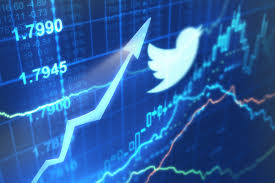
\includegraphics[scale = 0.5]{pics/tweetStock.jpeg}
        \end{figure}
\end{itemize}
\end{scriptsize}




\end{frame}

\begin{frame}{The NRC Emotion Lexicon}
\begin{scriptsize}\begin{itemize}
 \item A well known lexical resource for \textbf{automatically analysing} emotions from textual data is the \textbf{NRC word-emotion association lexicon} (NRC-10) \cite{Mohammad2013a}
 \item It contains more than 14,000 English words \textbf{manually annotated} according to ten non-exclusive \textbf{emotional} and \textbf{polarity categories}.
 \item Examples: \textbf{achieved} is mapped to \textbf{anticipation, joy, and trust}, and  \textbf{exile} is mapped into \textbf{anger, fear, and sadness}.
 
  \begin{figure}[htb]
	\centering
	 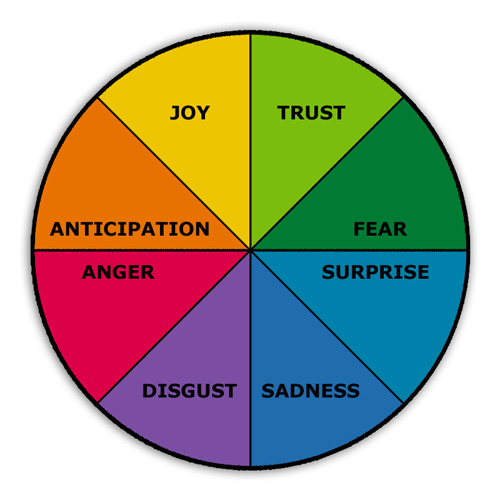
\includegraphics[scale=0.2]{pics/wheel_th.jpg}
\end{figure}
 
 \item  NRC-10 does not cover \textbf{informal expressions} used in Twitter. 
 \item It suffers from \textbf{limitations} for analysing emotions from tweets.
 \end{itemize}
\end{scriptsize}
\end{frame}






\begin{frame}{Proposal}
\begin{scriptsize}
\begin{itemize}
\item  We propose a method to \textbf{automatically expand} NRC-10 from  a target corpus of $10$ million tweets using a \textbf{multi-label classifier}. 

\item Multi-label classification techniques assign instances to \textbf{multiple non-exclusive classes} such as the ones provided by NRC-10.

\item All words from the corpus will be \textbf{mapped} into emotional categories.

\item We study which \textbf{combinations} of \textbf{word-level features} and \textbf{learning techniques} are most effective for this task. 
\end{itemize}
\end{scriptsize}

\end{frame}

\begin{frame}{Proposal (2)}

  \begin{figure}[htb]
	\centering
	 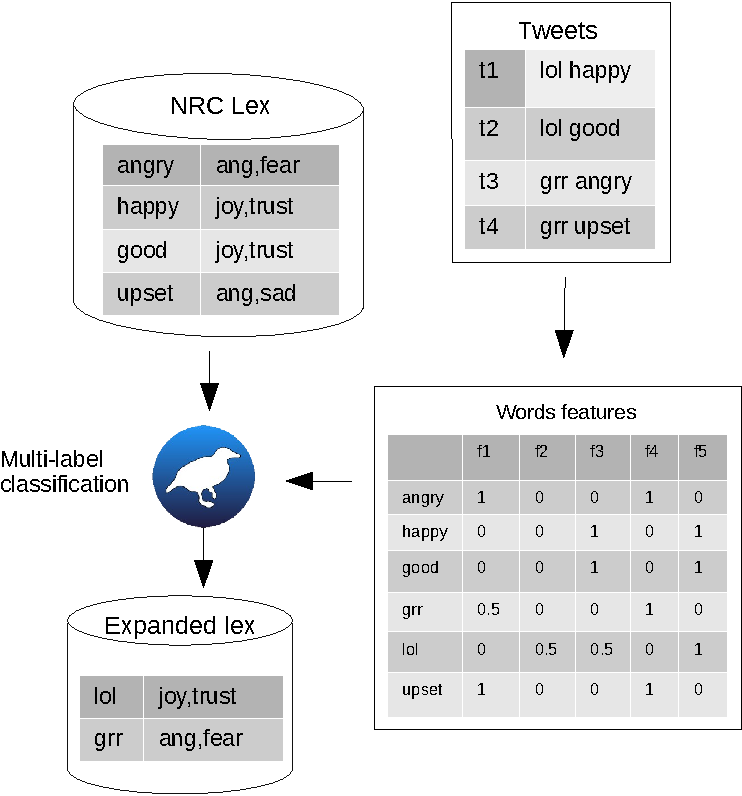
\includegraphics[scale=0.5]{pics/emo_model.pdf}
\end{figure}

\end{frame}



\begin{frame}{Previous work on emotion lexicon expansion}
\begin{scriptsize}

\begin{itemize} 
\item In~\cite{hashemo2015}, tweets annotated with hashtags corresponding to the six emotions: \textbf{\#anger}, \textbf{\#disgust}, \textbf{\#fear}, \textbf{\#happy}, \textbf{\#sadness}, and \textbf{\#surprise} were collected.

\item Example: Dad, close the door when you piss. No one wants to hear you're waterfall 	\textbf{\#disgust}.

\item The corpus was used for creating a \textbf{Twitter-specific emotion-association} lexicon using \textbf{Point-wise Mutual Information (PMI)} associations:

\begin{equation}
 \operatorname{PMI}(term_{1}, term_{2})= \log_{2} \left ( \frac{Pr(term_{1} \wedge term_{2})}{Pr(term_{1})Pr(term_{2})} \right )
\end{equation}

\begin{displaymath}
\operatorname{SoA}(w,e)= \operatorname{PMI}(w,e) - \operatorname{PMI}(w,\neg e)
\end{displaymath}
\end{itemize}



\end{scriptsize}
\end{frame}

\begin{frame}{Limitations of previous approach}
\begin{scriptsize}

\begin{itemize} 
\item Words that \textbf{do not co-occur} with those emotion-oriented hashtags will be \textbf{excluded}.
\item It would be \textbf{unsuitable} for creating \textbf{domain-specific emotion lexicons} for domains in which hashtags are not frequently used to express emotions such as \textbf{politics}. 
\item In contrast, our approach takes a \textbf{target corpus of unlabaled tweets} from any domain and a seed lexicon to perform the expansion. 
\end{itemize}

\end{scriptsize}
\end{frame}



\begin{frame}{Word-level features with the Tweet-Centroid Model}
\begin{scriptsize}
\begin{itemize} 
\item We treat a \textbf{whole tweet} as a word's context.
\item We model tweets as \textbf{vectors} calculated from the \textbf{content}.
\item We calculate word-level vectors based on the \textbf{centroids} of the \textbf{tweet-vectors} where a word occurs.
\end{itemize}
\end{scriptsize}
\end{frame}


\begin{frame}{From Tweet-level features to Word-level vectors}
\begin{scriptsize}
\begin{enumerate} 
\item \textbf{Word unigrams (UNI)}: based on an unigram frequency count.
\item \textbf{Brown clusters (BWN)}: in which the tweet is tagged according to low-dimensional Brown clusters of words. 
\item \textbf{POS n-grams (POS)}: in which the frequency of each POS unigram and bigram is counted.  
\item  \textbf{Distant Polarity (DP)}: in which a logistic regression model is trained from a corpus of tweets with positive \textbf{:)} and negative \textbf{:(} \textbf{emoticons} and applied to the tweet.
\end{enumerate}
\end{scriptsize}
\end{frame}



\begin{frame}{W2V word-level features}
\begin{scriptsize}
\begin{itemize}
\item  Word \textbf{embeddings} are low-dimensional continuous dense word vectors trained from document corpora.
\item We train \textbf{skip-gram word-embeddings (W2V)}  from the target corpus. 
\item  In this method, a \textbf{neural network} with one hidden layer is trained for predicting the words \textbf{surrounding a center word} within a window that is shifted along the target corpus.

  \begin{figure}[h]
        	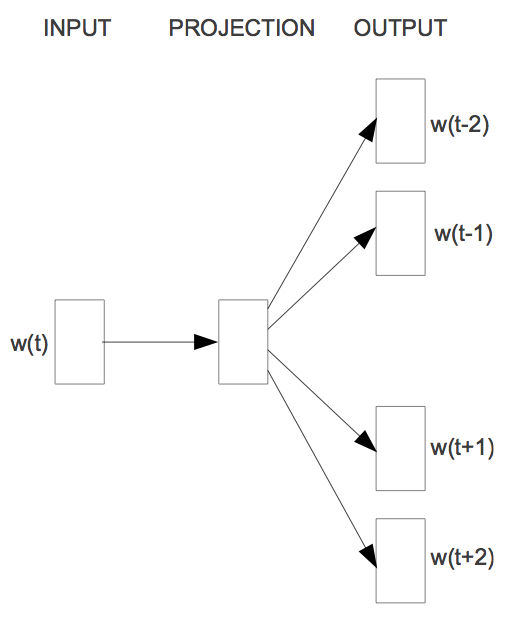
\includegraphics[scale = 0.45]{pics/skip-gram.png}
        \end{figure}

\end{itemize}
\end{scriptsize}
\end{frame}







\begin{frame}{Multi-Label Classification of word into Emotions}
\begin{scriptsize}
\begin{itemize}
\item The NRC-10 words occurring in the target corpus are labeled according to the \textbf{corresponding emotions}.
\item Their feature-vectors (UNI, BWN, POS, DP, W2V) are used for training a \textbf{multi-label classifier}. 
\item   The resulting classifier is used to classify the \textbf{remaining unlabeled words} into emotions. 
\end{itemize}
\end{scriptsize}
\end{frame}


\begin{frame}{Multi-Label Classification Models}
\begin{scriptsize}
\begin{enumerate}
\item \textbf{Binary Relevance (BR)}: in which one \textbf{separated binary classifier} is trained per label.
\item \textbf{Classifier Chains (CC)} \cite{read2011classifier}: in which the predictions for each binary classifier are \textbf{cascaded} as additional features along a random permutation of labels.
\item \textbf{Bayesian Classifier Chains (BCC)} \cite{ZaragozaSMBL11}: in which a Bayesian network that represents \textbf{dependency relations} between the labels is learned and used to build a \textbf{classifier chain}.  
\end{enumerate}
\end{scriptsize}
\end{frame}


\begin{frame}{Intrinsic Evaluation}
\begin{scriptsize}
\begin{itemize}
\item We compare the \textbf{micro-averaged F1} for the \textbf{ten affective} categories on the labeled words using \textbf{10-fold cross-validation}.
\item We use \textbf{logistic regression} as the \textbf{base learner} in the different models.
\item We compare different combinations of \textbf{features} and \textbf{classifiers}.
\begin{table}[htbp]
\begin{center}
\scalebox{0.8}{
\begin{tabular}{l|l@{\hspace{0.1cm}}l@{\hspace{0.1cm}}l@{\hspace{0.1cm}}l@{\hspace{0.1cm}}|l@{\hspace{0.1cm}}l@{\hspace{0.1cm}}l@{\hspace{0.1cm}}l@{\hspace{0.1cm}}|l@{\hspace{0.1cm}}l@{\hspace{0.1cm}}l@{\hspace{0.1cm}}l@{\hspace{0.1cm}}}
\hline
Classifier & \multicolumn{4}{c|}{BR} & \multicolumn{4}{c|}{CC} & \multicolumn{4}{c}{BCC}  \\ \hline
UNI (Baseline) &  0.389 & $\pm$ & 0.03 &  &  0.371 & $\pm$ & 0.03 &  & 0.378 & $\pm$ & 0.03 &   \\ \hline
UNI-BWN & 0.410 & $\pm$ & 0.03 & $\circ$ & 0.400 & $\pm$ & 0.03 & $\circ$   & 0.407 & $\pm$ & 0.03 & $\circ$  \\ 
UNI-BWN-POS &  0.411 & $\pm$ & 0.03 & $\circ$ &  0.405 & $\pm$ & 0.02 & $\circ$  & 0.407 & $\pm$ & 0.03 & $\circ$   \\ 
UNI-BWN-POS-DP &  0.433 & $\pm$ & 0.03 & $\circ$  &  0.427 & $\pm$ & 0.03 & $\circ$ & 0.432 & $\pm$ & 0.03 &  $\circ$  \\ 
UNI-BWN-POS-DP-W2V  &  0.477 & $\pm$ & 0.03 & $\circ$ &  0.474 & $\pm$ & 0.03 & $\circ$ & 0.478 & $\pm$ & 0.03 & $\circ$  \\ 
W2V  &  0.473 & $\pm$ & 0.03 & $\circ$ & 0.469 & $\pm$ & 0.03 & $\circ$ &  0.472 & $\pm$ & 0.03 &  $\circ$  \\ 
W2V-BWN  & 0.468 & $\pm$ & 0.03 & $\circ$ &  0.469 & $\pm$ & 0.03 & $\circ$ & 0.47 &  $\pm$ & 0.03 &   $\circ$  \\ 
W2V-BWN-POS  &   0.465 & $\pm$ & 0.03 & $\circ$ &  0.466 & $\pm$ & 0.03 & $\circ$ & 0.466 & $\pm$ & 0.02 &  $\circ$   \\ 
W2V-BWN-POS-DP  &  0.474 & $\pm$ & 0.03 & $\circ$ &   0.473 &  $\pm$ & 0.03 &  $\circ$ &  0.475 & $\pm$ & 0.03  & $\circ$  \\ 
W2V-DP  &  \textbf{0.479} & $\pm$ & 0.03 & $\circ$ &  \textbf{0.476} &  $\pm$ & 0.03 &  $\circ$ &  \textbf{0.479} & $\pm$ & 0.03  & $\circ$  \\ 

\end{tabular}}
\end{center} 
\end{table}
\item W2V-embeddings produce the \textbf{strongest} features!
\item There are \textbf{no clear differences} between multi-label models! 
\end{itemize}
\end{scriptsize}


\end{frame}


\begin{frame}{Expanded Lexicon}
\begin{figure}[htbp]
\begin{center}
\scalebox{0.7}{
\begin{tabular}{cccc}
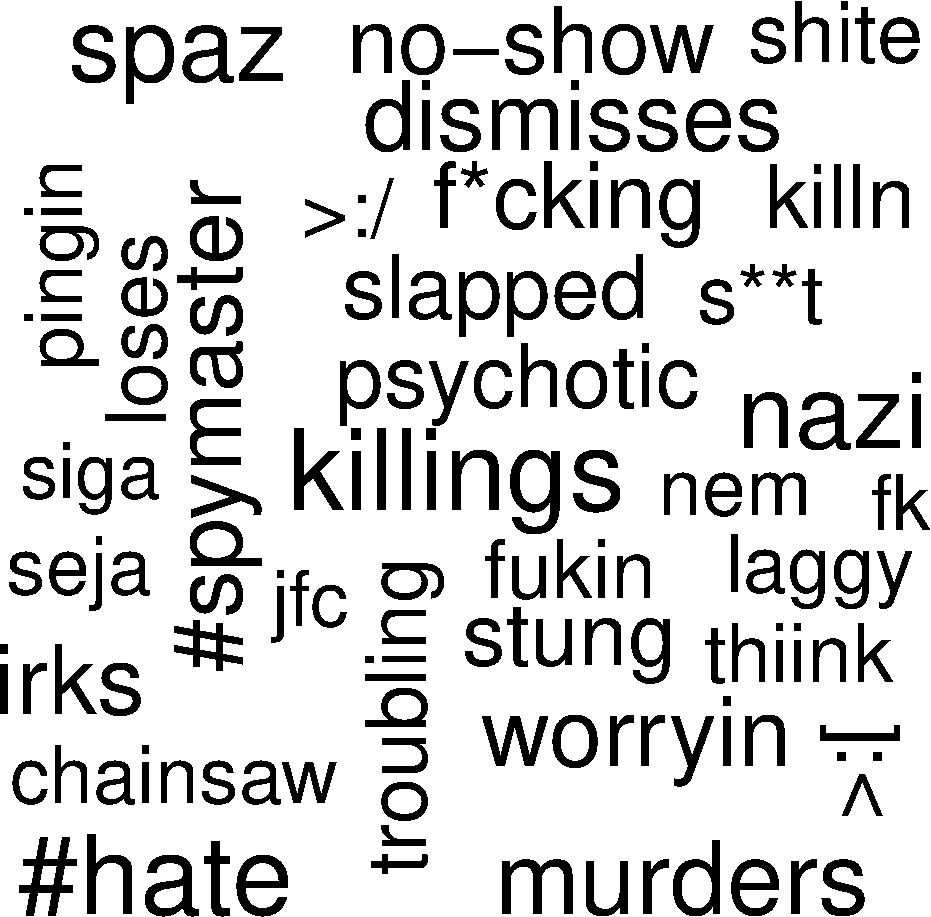
\includegraphics[scale=0.2]{../../emo_lex_naacl/anger.pdf} & 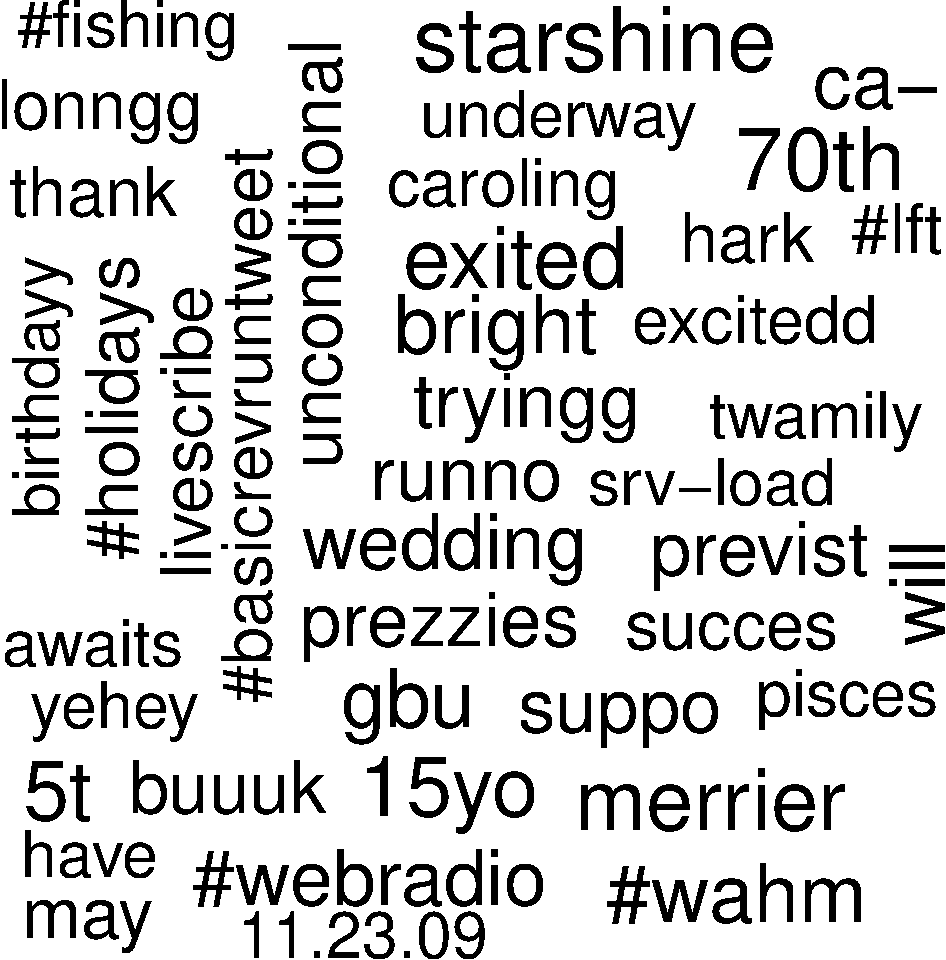
\includegraphics[scale=0.2]{../../emo_lex_naacl/ant.pdf} & 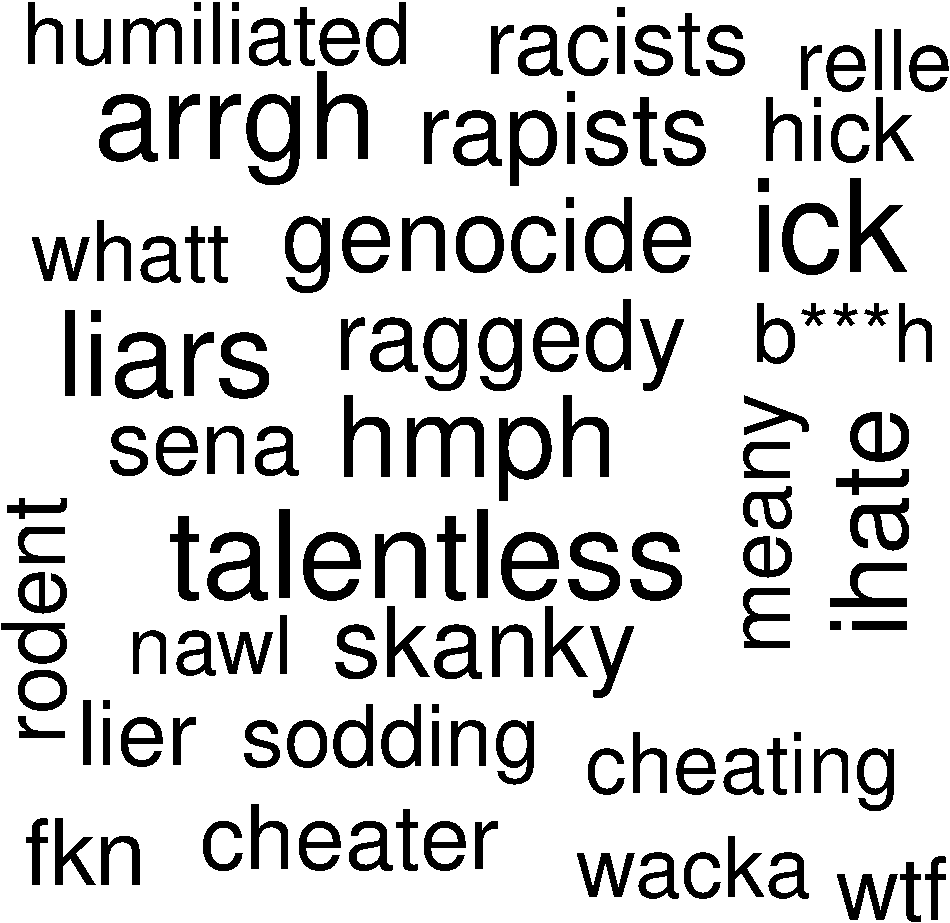
\includegraphics[scale=0.2]{../../emo_lex_naacl/disg.pdf} & 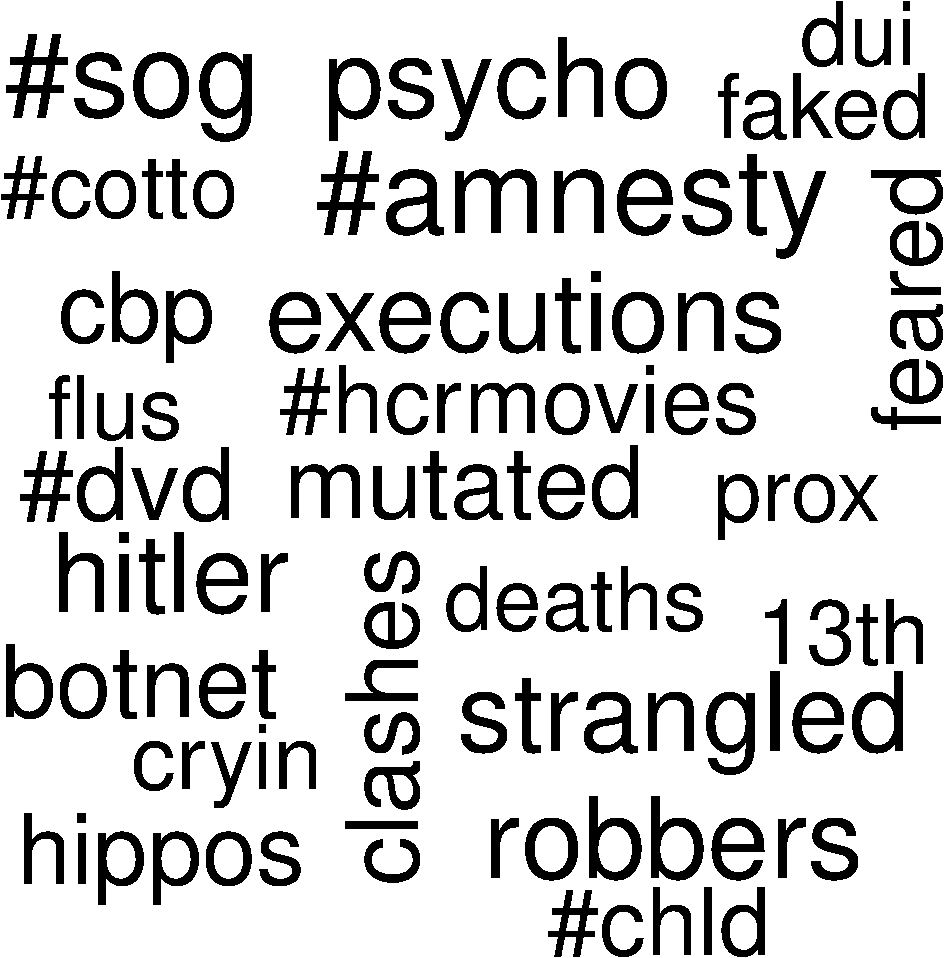
\includegraphics[scale=0.2]{../../emo_lex_naacl/fear.pdf} \\
anger & anticipation & disgust & fear\\[1mm] 
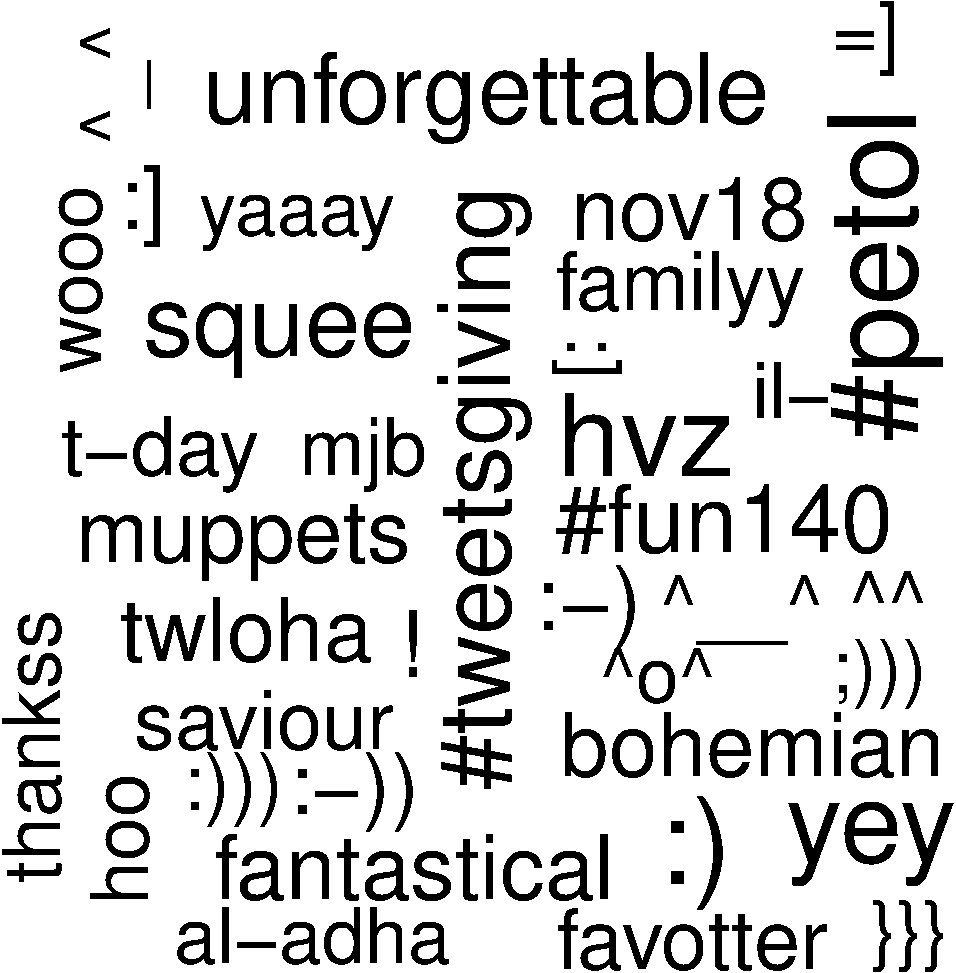
\includegraphics[scale=0.2]{../../emo_lex_naacl/joy.pdf} & 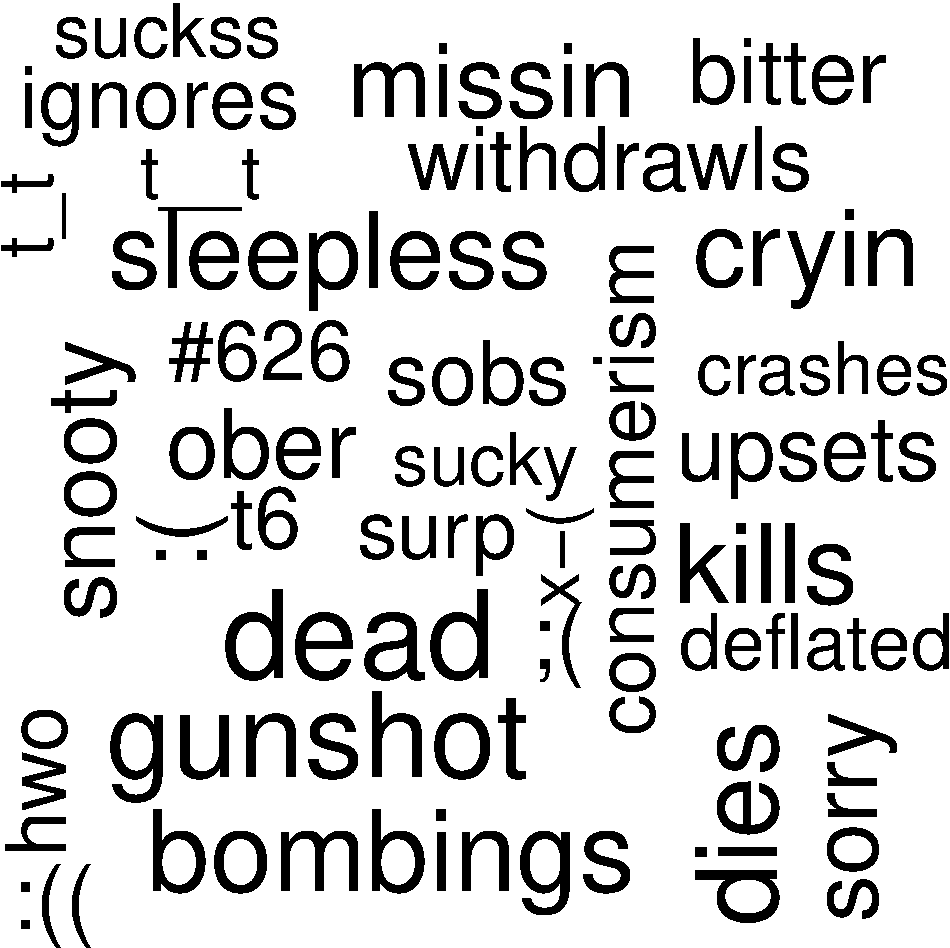
\includegraphics[scale=0.2]{../../emo_lex_naacl/sadness.pdf} & 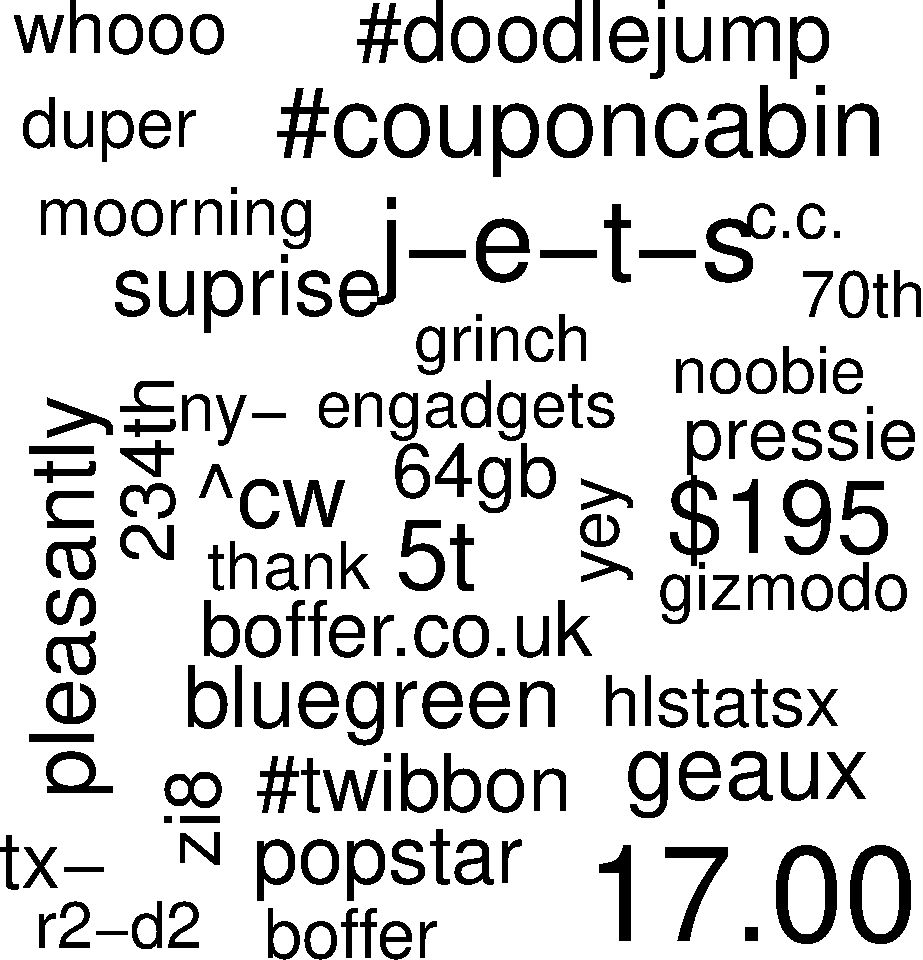
\includegraphics[scale=0.2]{../../emo_lex_naacl/surprise.pdf} & 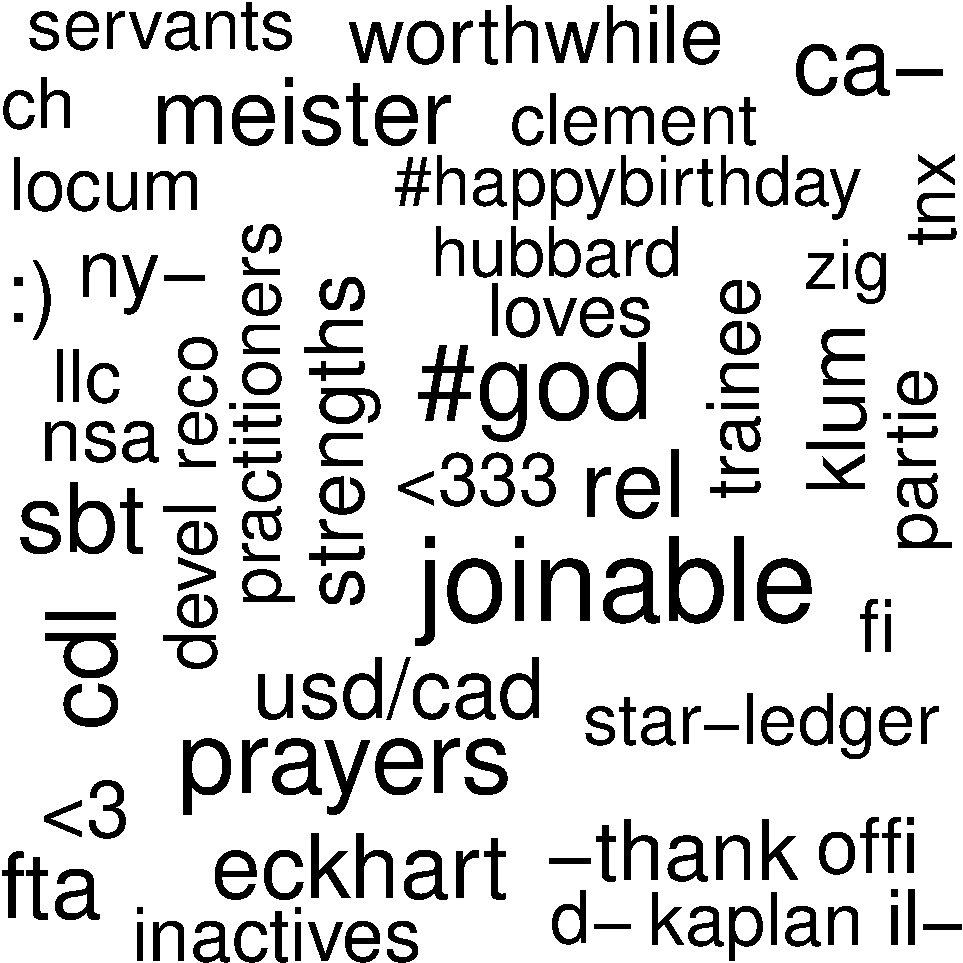
\includegraphics[scale=0.2]{../../emo_lex_naacl/trust.pdf} \\
joy & sadness & surprise & trust\\
\end{tabular}}
\end{center}
\end{figure}
\end{frame}


\begin{frame}{Extrinsic Evaluation}
\begin{scriptsize}
\begin{itemize}
\item We conduct an \textbf{extrinsic evaluation} by studying the usefulness of the expanded lexicons for classifying  Twitter messages annotated with \textbf{emotional hashtags}. 
\item We compare a \textbf{logistic regression} that uses \textbf{NRC-10 alone} with another one using  NRC-10 and \textbf{the expanded lexicon}.
\begin{table}[htbp]
\begin{center}
\scalebox{0.8}{
\begin{tabular}{l|ccc|ccc}
\hline
Lexicon & \multicolumn{3}{c|}{Kappa} & \multicolumn{3}{c}{AUC}  \\ \hline
 NRC-10 (alone)& \multicolumn{3}{c|}{0.0769} & \multicolumn{3}{c}{0.633}  \\ \hline 
 NRC-10+Expanded & BR & CC & BCC & BR & CC & BCC \\ \hline
UNI &   0.1912 & 0.2006 & 0.1977 & 0.711 & 0.714 & 0.713 \\  
UNI-BWN &  0.174 & 0.1783 & 0.176 & 0.708 & 0.712 &  0.711\\ 
UNI-BWN-POS &  0.1753 &  0.1767 & 0.1776 & 0.708 &  0.711 &  0.710 \\ 
UNI-BWN-POS-DP & 0.1803 & 0.1829 & 0.1835 & 0.713 & 0.715 & 0.714 \\ 
UNI-BWN-POS-DP-W2V & 0.1871 & 0.1966 &   0.1832 & 0.712  & 0.714  & 0.713 \\ 
W2V & \textbf{0.2234} &  \textbf{0.2256} & 0.2256 & 0.720 & \textbf{0.723} &  \textbf{0.723}  \\ 
W2V-BWN &  0.1988 &  0.2007 & 0.1974 & 0.713 & 0.715 & 0.715 \\ 
W2V-BWN-POS & 0.195 & 0.2012 &  0.1956 & 0.710 & 0.713 &  0.712 \\ 
W2V-BWN-POS-DP &  0.1994 & 0.2041 &  0.1992 & 0.714 & 0.715 & 0.715 \\ 
W2V-DP &  0.2228 & 0.2234 &   \textbf{0.2263} & \textbf{0.722}  & \textbf{0.723} & \textbf{0.723}  \\ \hline
\end{tabular}}
\end{center}
\end{table}
\item All the expanded lexicons are \textbf{substantially better} than using NRC-10 alone.
\item Lexicons created with CC and BCC are slightly better than the ones created using BR in most cases.  
\end{itemize}
\end{scriptsize}
\end{frame}



\begin{frame}{Conclusions}
\begin{scriptsize}
\begin{itemize}
\item The results obtained indicate that \textbf{low-dimensional word-embeddings} are better than distributional word-level features obtained by averaging \textbf{tweet-level features}.  
\item This is \textbf{aligned with recent findings} in NLP showing that representations learned from unlabeled data using \textbf{neural networks} outperform representations obtained from hand-crafted features.
\item This method could be used for creating \textbf{domain specific} emotion lexicons for elections or sport competitions.
\end{itemize}
\end{scriptsize}
\end{frame}




\begin{frame}{Future Work}
\begin{scriptsize}
\begin{itemize}
\item Study how to create \textbf{time-evolving} emotion lexicons from Twitter streams using \textbf{incremental} word-level representations and learning techniques. 
\item Explore \textbf{low-dimensional} dense word-embeddings obtained from the word-centroid model by training \textbf{auto-encoders} or restricted \textbf{Boltzman machines} on this representation.
\end{itemize}
\end{scriptsize}
\end{frame}





\begin{frame}
\frametitle{Questions?}
%\vspace{1.5cm}
\begin{center}\LARGE Thanks for your Attention!\\ \end{center}

\begin{columns}
\begin{column}{0.55\textwidth}
\begin{block}{Acknowledgments}
\begin{itemize}\tiny
	\item University of Waikato Doctoral Scholarship
	\item Machine Learning Group at the University of Waikato
	
\end{itemize}
\end{block}
\end{column}
\begin{column}{0.45\textwidth}
\vspace{1.5cm}

\begin{figure}[h!]
	\centering
	\includegraphics[scale=0.3]{../../img/waikato.png}
\end{figure}
\end{column}
\end{columns}

\end{frame}

\begin{frame}[allowframebreaks]\scriptsize
\frametitle{References}
\bibliography{../bio}
\bibliographystyle{apalike}
%\bibliographystyle{flexbib}
\end{frame}  


%%%%%%%%%%%%%%%%%%%%%%%%%%%

\end{document}
